Pour étudier la charge du condensateur, le professeur réalise le montage de la
Fig.~\ref{fig:svt_national_2016_normale_phys_ex2_1} constitué des éléments
suivants~:

\begin{itemize}
    \item un générateur idéal de courant qui alimente le circuit par un courant
          électrique d'intensité constante $I_{0}=\qty{2e-5}{\A}$~;
    \item un conducteur ohmique de résistance $R_{0}$~;
    \item un condensateur de capacité $C$~;
    \item un interrupteur $\mathrm{K}$.
\end{itemize}

À $t_{0}=0$, le professeur ferme l'interrupteur $\mathrm{K}$ et suit à l'aide
d'un dispositif convenable, les variations de la tension $u_{C}(t)$ aux bornes
du condensateur. La Fig.~\ref{fig:svt_national_2016_normale_phys_ex2_2}
représente la courbe obtenue.

\begin{minipage}{0.49\linewidth}
    \begin{figure}[H]
        \centering
        \raisebox{8mm}{%
        \begin{circuitikz}
            \newdimen\d \d=3cm
            \draw (0,0) coordinate (O)
                to[I,v^>=,name=I0] ++(0,\d)
                to[switch,l=$\mathrm{K}$] ++(\d,0)
                to[R,l=$R_{0}$] ++(\d,0)
                to[C,l_=$C$,v^<=$u_{C}$,i>^={ }] ++(0,-\d)
                to[short] (O);
            \fixedvlen{I0}{$I_{0}$}
        \end{circuitikz}}
        \caption{}
        \label{fig:svt_national_2016_normale_phys_ex2_1}
    \end{figure}
\end{minipage}
\begin{minipage}{0.49\linewidth}
\begin{figure}[H]
    \centering
    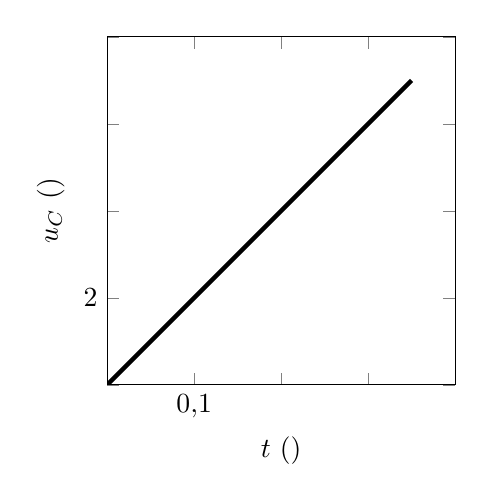
\begin{tikzpicture}[]
        \begin{axis}[
                width=6cm,height=6cm,
                xlabel=$t~(\unit{\s})$,ylabel=$u_{C}~(\unit{\V})$,
                xmin=0,xmax=0.4,
                ymin=0,ymax=8,
                variable=\t,
                domain=0:0.35,
                xticklabels={,,$0{,}1$,,},
                yticklabels={,,$2$,,},
            ]
            \addplot[ultra thick] {20*t};
        \end{axis}
    \end{tikzpicture}
    \caption{}
    \label{fig:svt_national_2016_normale_phys_ex2_2}
\end{figure}
\end{minipage}


\begin{enumerate}
    \item En exploitant la courbe, déterminer l'expression de la tension
          $u_{C}(t)$.
    \item \label{item:culcul_C}
          Montrer que $C=\qty{1}{\uF}$.
\end{enumerate}
